%% (Master) Thesis template
% Template version used: v1.4
%
% Largely adapted from Adrian Nievergelt's template for the ADPS
% (lecture notes) project.


%% We use the memoir class because it offers a many easy to use features.
\documentclass[11pt,a4paper,titlepage]{memoir}

%% Packages
%% ========

%% LaTeX Font encoding -- DO NOT CHANGE
\usepackage[OT1]{fontenc}

%% Babel provides support for languages.  'english' uses British
%% English hyphenation and text snippets like "Figure" and
%% "Theorem". Use the option 'ngerman' if your document is in German.
%% Use 'american' for American English.  Note that if you change this,
%% the next LaTeX run may show spurious errors.  Simply run it again.
%% If they persist, remove the .aux file and try again.
\usepackage[english]{babel}

%% Input encoding 'utf8'. In some cases you might need 'utf8x' for
%% extra symbols. Not all editors, especially on Windows, are UTF-8
%% capable, so you may want to use 'latin1' instead.
\usepackage[utf8]{inputenc}

%% This changes default fonts for both text and math mode to use Herman Zapfs
%% excellent Palatino font.  Do not change this.
\usepackage[sc]{mathpazo}

%% The AMS-LaTeX extensions for mathematical typesetting.  Do not
%% remove.
\usepackage{amsmath,amssymb,amsfonts,mathrsfs}

%% NTheorem is a reimplementation of the AMS Theorem package. This
%% will allow us to typeset theorems like examples, proofs and
%% similar.  Do not remove.
%% NOTE: Must be loaded AFTER amsmath, or the \qed placement will
%% break
\usepackage[amsmath,thmmarks]{ntheorem}

%% LaTeX' own graphics handling
\usepackage{graphicx}

%% Better arrange figures.
\usepackage{float}

%% Be able to draw svg's.
\usepackage{svg}

%% We unfortunately need this for the Rules chapter.  Remove it
%% afterwards; or at least NEVER use its underlining features.
\usepackage{soul}

%% This allows you to add .pdf files. It is used to add the
%% declaration of originality.
\usepackage{pdfpages}

%% Some more packages that you may want to use.  Have a look at the
%% file, and consult the package docs for each.
%% See the TeXed file for more explanations

%% [OPT] Multi-rowed cells in tabulars
%\usepackage{multirow}

%% [REC] Intelligent cross reference package. This allows for nice
%% combined references that include the reference and a hint to where
%% to look for it.
\usepackage{varioref}

%% [OPT] Easily changeable quotes with \enquote{Text}
%\usepackage[german=swiss]{csquotes}

%% [REC] Format dates and time depending on locale
\usepackage{datetime}

%% [OPT] Provides a \cancel{} command to stroke through mathematics.
%\usepackage{cancel}

%% [NEED] This allows for additional typesetting tools in mathmode.
%% See its excellent documentation.
\usepackage{mathtools}

%% [ADV] Conditional commands
%\usepackage{ifthen}

%% [OPT] Manual large braces or other delimiters.
%\usepackage{bigdelim, bigstrut}

%% [REC] Alternate vector arrows. Use the command \vv{} to get scaled
%% vector arrows.
\usepackage[h]{esvect}

%% [NEED] Some extensions to tabulars and array environments.
\usepackage{array}

%% [OPT] Postscript support via pstricks graphics package. Very
%% diverse applications.
%\usepackage{pstricks,pst-all}

%% [?] This seems to allow us to define some additional counters.
%\usepackage{etex}

%% [ADV] XY-Pic to typeset some matrix-style graphics
%\usepackage[all]{xy}

%% [OPT] This is needed to generate an index at the end of the
%% document.
%\usepackage{makeidx}

%% [OPT] Fancy package for source code listings.  The template text
%% needs it for some LaTeX snippets; remove/adapt the \lstset when you
%% remove the template content.
\usepackage{listings}
\lstset{language=TeX,basicstyle={\normalfont\ttfamily}}

%% [REC] Fancy character protrusion.  Must be loaded after all fonts.
\usepackage[activate]{pdfcprot}

%% [REC] Nicer tables.  Read the excellent documentation.
\usepackage{booktabs}


%% Our layout configuration.  DO NOT CHANGE.
%% Memoir layout setup

%% NOTE: You are strongly advised not to change any of them unless you
%% know what you are doing.  These settings strongly interact in the
%% final look of the document.

% Dependencies
\usepackage{ETHlogo}

% Turn extra space before chapter headings off.
\setlength{\beforechapskip}{0pt}

\nonzeroparskip
\parindent=0pt
\defaultlists

% Chapter style redefinition
\makeatletter

\if@twoside
  \pagestyle{Ruled}
  \copypagestyle{chapter}{Ruled}
\else
  \pagestyle{ruled}
  \copypagestyle{chapter}{ruled}
\fi
\makeoddhead{chapter}{}{}{}
\makeevenhead{chapter}{}{}{}
\makeheadrule{chapter}{\textwidth}{0pt}
\copypagestyle{abstract}{empty}

\makechapterstyle{bianchimod}{%
  \chapterstyle{default}
  \renewcommand*{\chapnamefont}{\normalfont\Large\sffamily}
  \renewcommand*{\chapnumfont}{\normalfont\Large\sffamily}
  \renewcommand*{\printchaptername}{%
    \chapnamefont\centering\@chapapp}
  \renewcommand*{\printchapternum}{\chapnumfont {\thechapter}}
  \renewcommand*{\chaptitlefont}{\normalfont\huge\sffamily}
  \renewcommand*{\printchaptertitle}[1]{%
    \hrule\vskip\onelineskip \centering \chaptitlefont\textbf{\vphantom{gyM}##1}\par}
  \renewcommand*{\afterchaptertitle}{\vskip\onelineskip \hrule\vskip
    \afterchapskip}
  \renewcommand*{\printchapternonum}{%
    \vphantom{\chapnumfont {9}}\afterchapternum}}

% Use the newly defined style
\chapterstyle{bianchimod}

\setsecheadstyle{\Large\bfseries\sffamily}
\setsubsecheadstyle{\large\bfseries\sffamily}
\setsubsubsecheadstyle{\bfseries\sffamily}
\setparaheadstyle{\normalsize\bfseries\sffamily}
\setsubparaheadstyle{\normalsize\itshape\sffamily}
\setsubparaindent{0pt}

% Set captions to a more separated style for clearness
\captionnamefont{\sffamily\bfseries\footnotesize}
\captiontitlefont{\sffamily\footnotesize}
\setlength{\intextsep}{16pt}
\setlength{\belowcaptionskip}{1pt}

% Set section and TOC numbering depth to subsection
\setsecnumdepth{subsection}
\settocdepth{subsection}

%% Titlepage adjustments
\pretitle{\vspace{0pt plus 0.7fill}\begin{center}\HUGE\sffamily\bfseries}
\posttitle{\end{center}\par}
\preauthor{\par\begin{center}\let\and\\\Large\sffamily}
\postauthor{\end{center}}
\predate{\par\begin{center}\Large\sffamily}
\postdate{\end{center}}

\def\@advisors{}
\newcommand{\advisors}[1]{\def\@advisors{#1}}
\def\@department{}
\newcommand{\department}[1]{\def\@department{#1}}
\def\@thesistype{}
\newcommand{\thesistype}[1]{\def\@thesistype{#1}}

\renewcommand{\maketitlehooka}{\noindent\ETHlogo[2in]}

\renewcommand{\maketitlehookb}{\vspace{1in}%
  \par\begin{center}\Large\sffamily\@thesistype\end{center}}

\renewcommand{\maketitlehookd}{%
  \vfill\par
  \begin{flushright}
    \sffamily
    \@advisors\par
    \@department, ETH Z\"urich
  \end{flushright}
}

\checkandfixthelayout

\setlength{\droptitle}{-48pt}

\makeatother

% This defines how theorems should look. Best leave as is.
\theoremstyle{plain}
\setlength\theorempostskipamount{0pt}

%%% Local Variables:
%%% mode: latex
%%% TeX-master: "thesis"
%%% End:


%% Theorem environments.  You will have to adapt this for a German
%% thesis.
%% Theorem-like environments

%% This can be changed according to language. You can comment out the ones you
%% don't need.

\numberwithin{equation}{chapter}

%% German theorems
%\newtheorem{satz}{Satz}[chapter]
%\newtheorem{beispiel}[satz]{Beispiel}
%\newtheorem{bemerkung}[satz]{Bemerkung}
%\newtheorem{korrolar}[satz]{Korrolar}
%\newtheorem{definition}[satz]{Definition}
%\newtheorem{lemma}[satz]{Lemma}
%\newtheorem{proposition}[satz]{Proposition}

%% English variants
\newtheorem{theorem}{Theorem}[chapter]
\newtheorem{example}[theorem]{Example}
\newtheorem{remark}[theorem]{Remark}
\newtheorem{corollary}[theorem]{Corollary}
\newtheorem{definition}[theorem]{Definition}
\newtheorem{lemma}[theorem]{Lemma}
\newtheorem{proposition}[theorem]{Proposition}

%% Proof environment with a small square as a "qed" symbol
\theoremstyle{nonumberplain}
\theorembodyfont{\normalfont}
\theoremsymbol{\ensuremath{\square}}
\newtheorem{proof}{Proof}
%\newtheorem{beweis}{Beweis}


%% Helpful macros.
%% Custom commands
%% ===============

%% Special characters for number sets, e.g. real or complex numbers.
\newcommand{\C}{\mathbb{C}}
\newcommand{\K}{\mathbb{K}}
\newcommand{\N}{\mathbb{N}}
\newcommand{\Q}{\mathbb{Q}}
\newcommand{\R}{\mathbb{R}}
\newcommand{\Z}{\mathbb{Z}}
\newcommand{\X}{\mathbb{X}}

%% Fixed/scaling delimiter examples (see mathtools documentation)
\DeclarePairedDelimiter\abs{\lvert}{\rvert}
\DeclarePairedDelimiter\norm{\lVert}{\rVert}

%% Use the alternative epsilon per default and define the old one as \oldepsilon
\let\oldepsilon\epsilon
\renewcommand{\epsilon}{\ensuremath\varepsilon}

%% Also set the alternate phi as default.
\let\oldphi\phi
\renewcommand{\phi}{\ensuremath{\varphi}}


\graphicspath{ {./images/} }


%% Make document internal hyperlinks wherever possible. (TOC, references)
%% This MUST be loaded after varioref, which is loaded in 'extrapackages'
%% above.  We just load it last to be safe.
\usepackage[linkcolor=black,colorlinks=true,citecolor=black,filecolor=black]{hyperref}


%% Document information
%% ====================

\title{Multi-model disentanglement of object representations}
\author{Eric Stavarache}
\thesistype{Research Project Thesis}
\advisors{Advisors: Frederik Benzing, Asier Mujika}
\department{Department of Computer Science}
\date{July 19, 2019}

\begin{document}

\frontmatter
\raggedbottom

%% Title page is autogenerated from document information above.  DO
%% NOT CHANGE.
\begin{titlingpage}
  \calccentering{\unitlength}
  \begin{adjustwidth*}{\unitlength-24pt}{-\unitlength-24pt}
    \maketitle
  \end{adjustwidth*}
\end{titlingpage}

%% The abstract of your thesis.  Edit the file as needed.
\begin{abstract}
  Being able to decompose a scene into elementary components is a mark of
intelligence. In this work we present a novel approach to learning a
disentangled representation of scenes, by having several VAE's wired up in
parallel, with each of them representing a different type of object.
\end{abstract}

%% TOC with the proper setup, do not change.
\cleartorecto
\tableofcontents
\mainmatter

\chapter{Introduction}

Humans reason about the surrounding world by decomposing it into orthogonal components.
The idea of an object is decoupled from the qualities of the object: it is very
easy for us to imagine a pink elephant, even though we have never observed such
an animal, and these two words suffice for us to imagine a visual scene.
The words are a latent representation of the scene.

Variational Autoencoders (VAE) \cite{bib:vae_paper} are a powerful framework for
learning latent representations. Much work has already been done on disentangled
representations, where we require that any two latent variables are uncorrelated.

Our work focuses on model-based disentanglement of objects. In particular, for
each type of object we would like to have a VAE which is trained to recognise
it: in a normal setting, we could have one VAE which represents chairs, another
VAE which represents tables, and so on.
We will call our approach the \textbf{ParallelVAE}.

\chapter{Related work}

Most similar in spirit is the \cite{bib:monet}, where a single VAE model
iteratively recognises objects from a scene by using attention masks.
The main difference is that the MONet uses a single VAE for all objects, whereas
we use multiple VAE's in parallel.
Another similar idea is contained in \cite{bib:iodine}, where they have a single
VAE which tries to model the scene, and where they iteratively refine the latent
parameters.

\chapter{Model}

\section{ParallelVAE}


The ParallelVAE network tries to reconstruct a scene by feeding the image to some
VAE's connected in parallel, whereby each VAE models a separate part of the scene.

Let us say that there are $K$ VAE's, where each of them tries to model a
different object.
Then the image $X$ will be fed independently to
each of them.

Each VAE will then model a distribution over the latent variables,
$q_{\theta_k}(\textbf{z}_k | \textbf{X})$.

By sampling from these distributions, they will generate two outputs of
the same size as the image: $\hat{X}_k$, which is the $k$'th model
reconstruction of the image, and $\hat{m}_{k}$, which is a confidence mask.

This confidence mask represents how sure a VAE is about its output for a given
pixel. Higher confidence means that the pixel is part of an object which is of
the type the VAE is modelling.

These confidence masks are produced by first having the models generate some
``raw'' confidence values, and then taking a pixel-wise softmax across all of
the $k$ models.

Thus, the masks are a probability distribution, where for each pixel we have
what is the probability that it belongs to an object modelled by a VAE:

$\sum_{i = 1}^{k} \hat{m}_{k} = \textbf{1}$.

\begin{figure}
  \caption{A diagram of how the model operates.}
  \includegraphics[scale=0.7]{model.png}
\end{figure}

Our loss function is

\begin{align*}
  \mathcal{L}(X; \theta _1, ..., \theta_k) =
  & \sum_{i = 1}^{k}
    (\hat{X}_{i} - X)
    ^2
    \odot \hat{m}_{i}
  \\
  & +
  \beta \sum_{i = 1}^{k} D_{KL} [ q_{\theta_k} (\textbf{z}_k | \textbf{X}) ||
  \mathcal{N}(0, \mathbf{I}) ]
  \\
  & +
  \gamma \cdot - \log (
  \frac{1} {\log{K}}
  \cdot - \hat{m} \log {\hat{m}}
  )
\end{align*}

The first term of the loss is a $L_2$ loss weighted by each model's confidence.
The intuition behind this is that the more responsability a VAE takes for
drawing a certain pixel, the more it should be penalized for making mistakes.

The second term is the standard KL loss term, weighted by a $\beta$
hyperparameter, as first introduced in \cite{bib:betavae}.
We note that the KL loss can be interpreted as how much information is stored in
the bottleneck; the presence of this term means that in an optimal solution, no
information should be duplicated between VAE's: if one of them remembers that
there is a chair in the picture, then another VAE remembering the same thing
would only increase the KL loss, while not providing any additional
reconstruction gains.

The last term is our original contribution, which is a cross-entropy loss.
The idea is that the VAE's should try to be unassuming, and they should incur a
cost if they decide to take on a lot of responsability for representing a pixel.
We have the $-\hat{m} \log {\hat{m}}$ term, which is the normal cross-entropy,
where we interpret the masks as component-wise distributions over VAE's.
We divide it by the maximal value it can take ($\log{K}$, where $K$ is the
number of VAE's) in order to obtain a value between $0$ and $1$.
We want to penalize situations where one VAE takes over everything, and in these
situations the cross-entropy would be close to $0$. As such, we take the
negative log of the normalized cross-entropy.
This whole term is weighted by another hyperparameter, $\gamma$.
One reason for our introduction of this loss is that, without it, if a VAE
would ``take over'' a part of the image (have really high confidence), then the
other VAE's would have really small gradients, and they would never have the
chance to learn. With this loss, VAE's are very heavily penalized for being
overly confident.


We compare this with the approach of \cite{bib:monet}, where they have a single
VAE which tries to model all objects, whereas we have a single VAE for each
object type.
Furthermore, in their model, the VAE is instructed what to model by the U-Net
attention mask, whereas in our approach each VAE decides ``independently'' what
to learn. In our approach, the only communication happening between the VAE's is
via the softmax operation of the confidence masks.

\subsection{Training}

In order to train our ParallelVAE, we split the training into multiple stages.
Let us suppose that we know there are $K$ item types, and also our ParallelVAE
is composed of $K$ VAE's.
Then the training program is:

\begin{enumerate}
\item In stage 0, VAE-0 trains on reconstructing images containing
  only the item $0$. The other models is active (so they are contributing
  to the confidence masks), but their weights are frozen, and only
  VAE-0 is learning.
\item In stage 1, VAE-1 trains on images containing items $0$ and $1$ . In this
time, VAE-0, VAE-2, ..., VAE-k are frozen, \textit{however} they are still
contributing to the confidence masks.
Because of this, places where the item $0$ appears are
already assigned high confidence values by VAE-0, and so VAE-1 will not be
motivated to learn them. On the other hand, places where item $1$ appears will
not be recognised by VAE-0, and so VAE-1 will learn them.

\item ...

\item In stage $2n$, VAE-n trains on the item $n$, with the others frozen.
\item In stage $2n + 1$, VAE-0, VAE-1, ..., VAE-n train together on images
  of items $0$, $1$, ..., $n$.
\end{enumerate}


\subsection{Intuition}

We will now try to provide some explanations for why the ParallelVAE model
previously described should work.

Because of the KL loss, an optimal model should not duplicate information. 
One instance when this happen is if each VAE learns a different object.
Another instance is that one VAE learns everything, and the others do nothing.
This scenario can occur if, while training, one VAE just has very high
confidence, and so the others never have enough gradients in order to learn
anything.
In order to avoid this happening, and to encourage the models to split, we
introduced the entropy loss -- paying a price for taking responsability. This
way, the solution when one model takes care of everything is no longer optimal.

Multiple VAE's training all at the same time would pose great optimization
instability, so in order to improve stability, we decided to go for the
stage-based training approach, so that each VAE is given an opportunity to learn
its object.


\chapter{Results}

For our experiments, we have taken a supervised approach to training the models.

\section{MNIST}

In order to test our idea, we began with the MNIST dataset.
To make the task more challenging, and to allow decomposition via objects, we
construct our training data by putting two digits side-by-side, where the digits
that we use are the same as the number of VAE's (so for 4 VAE's, we will use the
digits $0, 1, 2, 3$).
We also include the ``empty digit'' (which is just an empty black square). This
is so that the VAE's also encounter scenarios when it is optimal to not output anything.

\subsection{2-MNIST}

At the start, we set up only 2 VAE's in parallel, where we want that VAE-0 learns to
recognise and model the digit 0, and VAE-1 models digit 1.

In order to accomplish this, we split the training into two stages:

\begin{enumerate}
  \item In stage 0, VAE-0 trains on reconstructing images containing
    only the digit $0$. The other model is active (so they are contributing
    to the confidence masks), but its weights are frozen, and only
    VAE-0 is learning.
  \item In stage 1, VAE-1 trains on images containing digits $0$ and $1$ (so of
    the two slots, each digit is sampled independently). In this time, VAE-0 is
    frozen, \textit{however} it is still contributing to the confidence masks.
    Because of this, places where the digit $0$ appears are already assigned
    high confidence values by VAE-0, and so VAE-1 will not be motivated to learn
    them. On the other hand, places where digit 1 appears will not be recognised
    by VAE-0, and so VAE-1 will learn them.
\end{enumerate}

\begin{figure}[]
  \label{fig:2mnist}
  \caption{Results of training on 2-MNIST.
    Each picture has 6 rows: first row is input image $X$, second row is
    confidence mask of VAE-0 $\hat{m}_{0}$, third row is reconstruction of VAE-0
    $\hat{X}_{0}$, fourth row is $\hat{m}_{1}$, fifth row is $\hat{X}_{1}$, and
    last row is weighted reconstruction.
  }
  \centering
  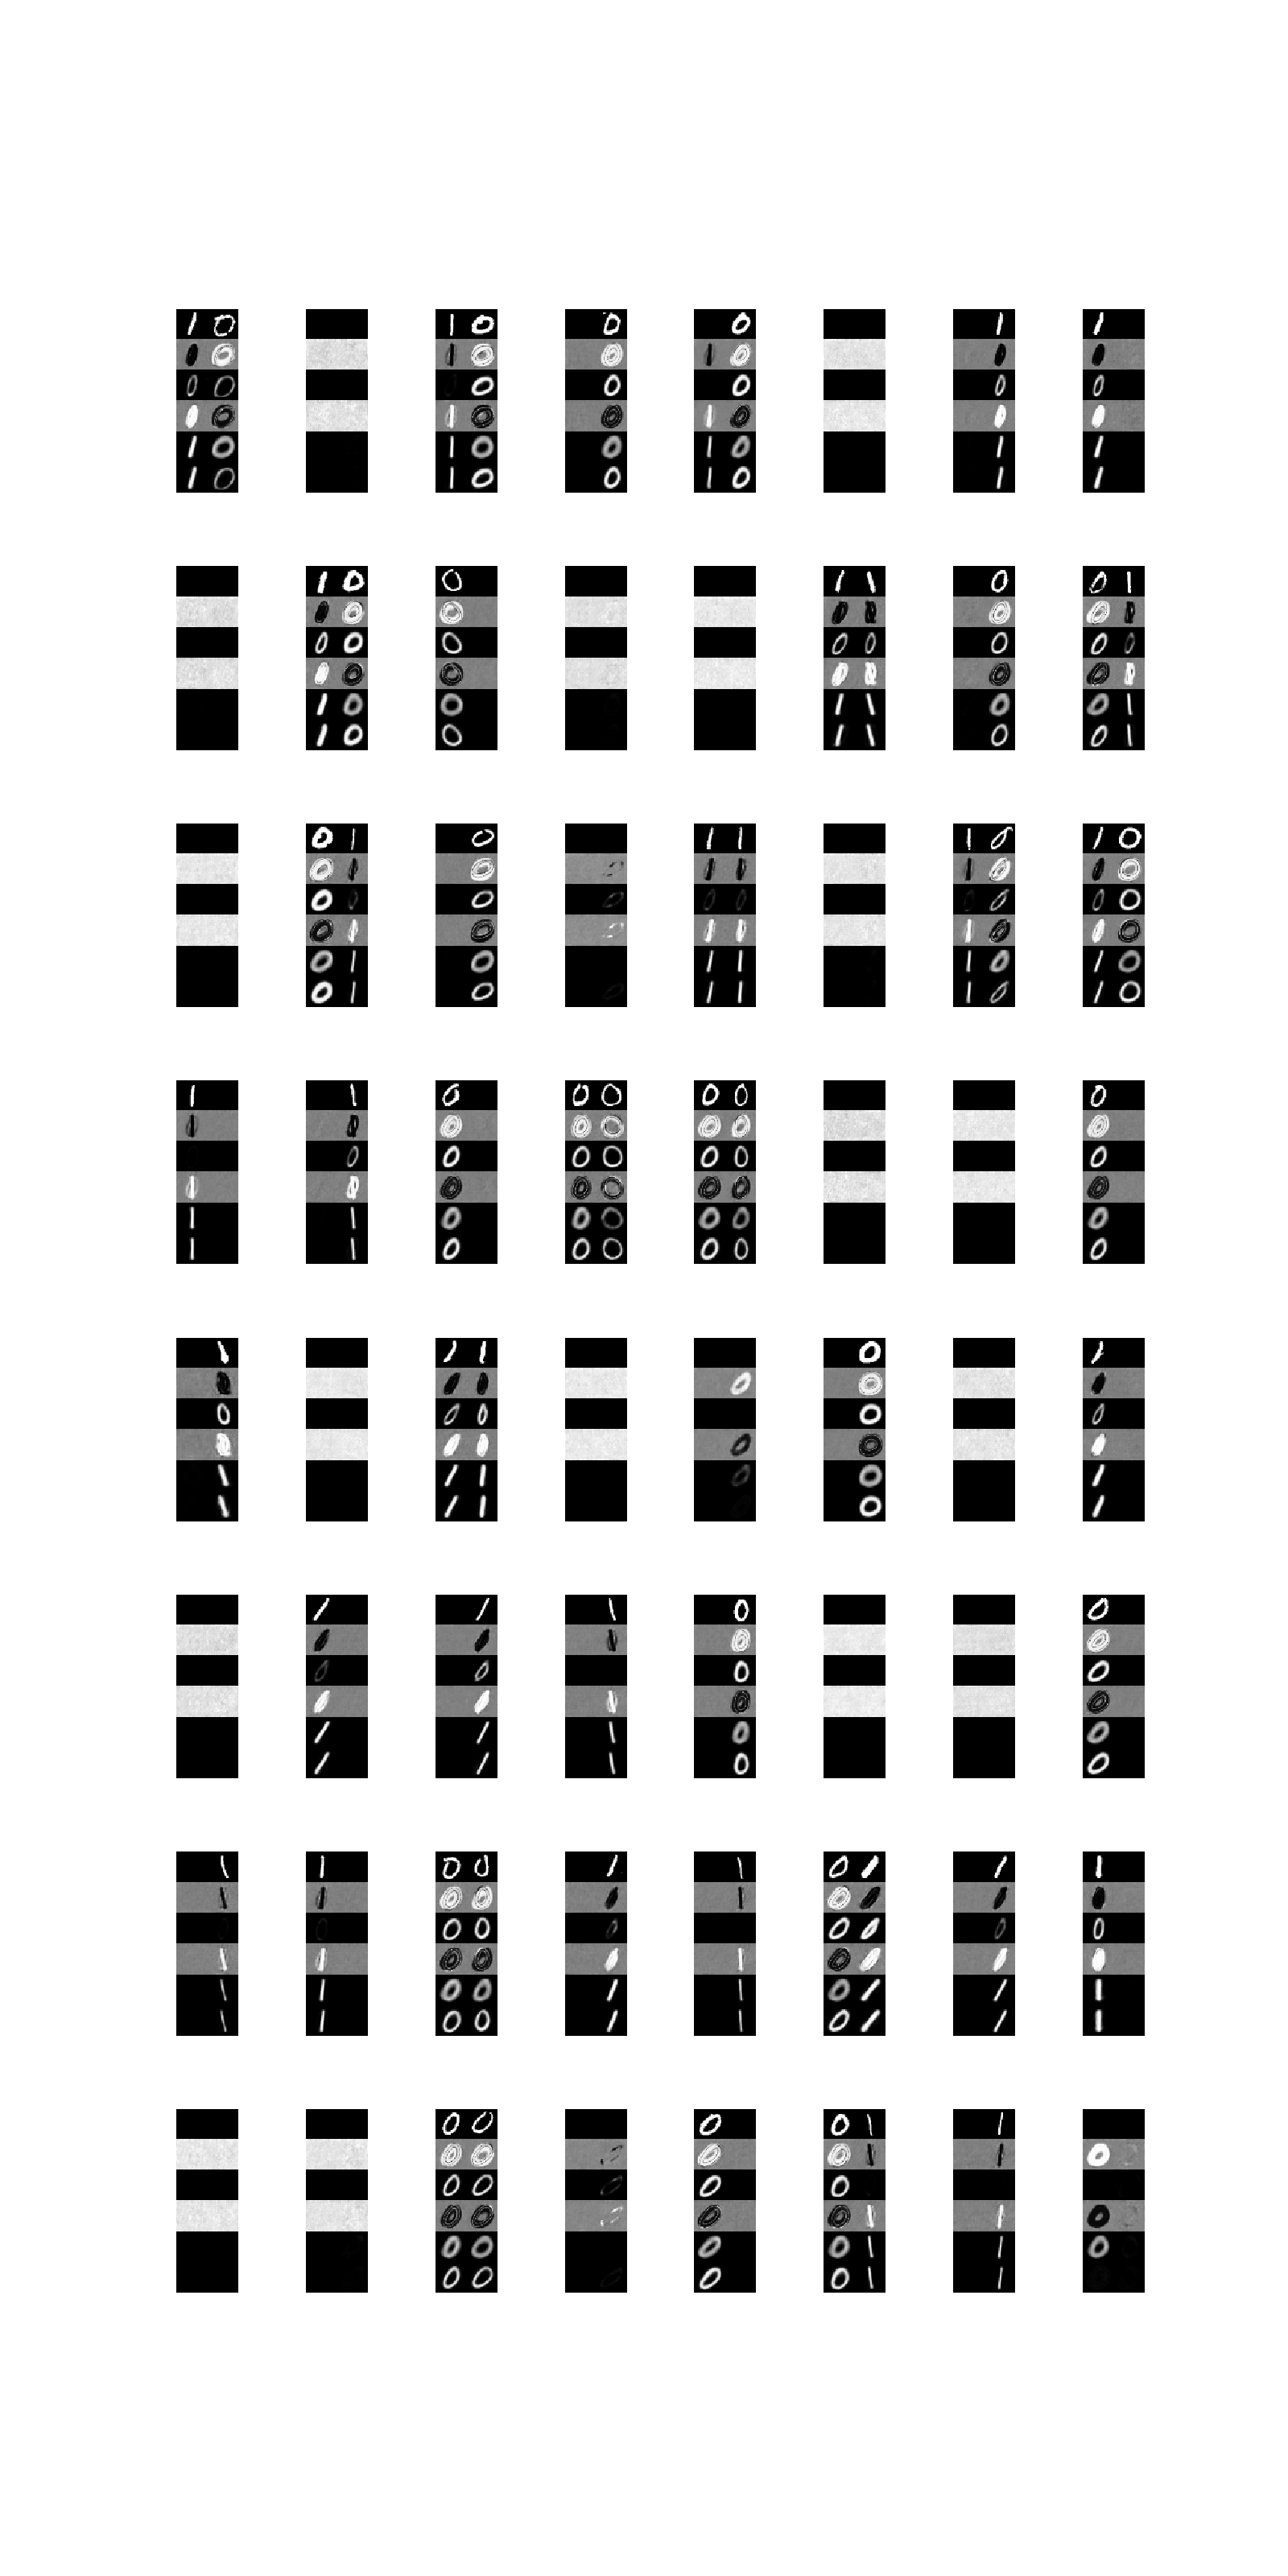
\includegraphics[scale=0.3]{init_progress.png}
\end{figure}

As we can see in figure \ref{fig:2mnist}, we have the desired effect: VAE 0 has
high confidences (indicated by very white portions of the confidence mask) where
the digit 0 appears, and has VAE 1 has high confidences where the digit 1 appears.

We note that there are cases when, even though VAE 0 has low confidence, it
still draws a 0. This is because it was trained only on zeroes, so when
encountering a digit 1 it does the only thing it knows how to do: output a 0.
Similarly, VAE 1 draws very generic zeroes when the input digit is a 0. Since it
was trained on both images of 0 and 1, it has had a chance to learn how a
generic 0 looks like. Furthermore, it only takes one bit of information to store
if the input is a $0$ (which is then included in the KL-loss), but it has a lot
to gain by making its reproduction closer to the original image (which is the
first term in the overall loss function).

After this experiment, we then proceeded to see what would happen with $5$ VAE's
in parallel.

\subsection{5-MNIST}

For this dataset, we again have the same two digit side-by-side training data.
However, we now have $5$ VAE's wired up together, where again we would want that
VAE $i$ learns to model digit $i$.

The training is done analogous to 2-MNIST, in $5$ stages, where in stage $k$
model $k$ is learning by looking at images containing digits $0, 1, ..., k$, and
all of the other models are frozen (but still contributing to the confidences).

\begin{figure}[]
  \label{fig:5mnist}
  \caption{Results of training on 5-MNIST.
    Each picture has 12 rows: first row is input image $X$, last row is
    reconstructed image.
    In between, each adjacent pair of rows represents the confidences
    $\hat{m}_k$ and the reconstructions $\hat{X}_k$ for each of the $K = 5$ VAE's.
    Note that even though the digit $5$ appears as part of the input, none of
    the models were trained on it: this is just test data. We include it only to
    see how models generalize to unseen digits.
  }
  \centering
  \includegraphics[scale=0.3]{5-mnist.png}
\end{figure}

From figure \ref{fig:5mnist}, we can see that the model achieves decent
reconstructions on the digits which it was trained on, although not as good as
we would expect.

Again, we observe that when a digit $4$ appears, only the last model has high
confidences, and produces a good reconstruction; the other models generate a
digit which they have learned, which minimizes the $L_2$ loss.

For digit $5$, we observe that the model with the closest digit (in $L_2$ norm)
has high confidence: sometimes the model for $2$, and sometimes the model for
$3$.

\subsection{Together training}


Here we introduce ``together-training'', where we differentiate between two
types of training stages: individual-training stages, and together-training
stages. Our motivation for this modification is that, afer is that after VAE $k$
has learned to represent the digit $k$ the other models should then learn to not
activate in case digit $k$ is in the input.


In the previous figures, a model which was trained for digits up to $k$ tends to
have low confidence when it receives as input one of the digits $0$, ..., $k -
1$ (which it has seen while training, and it was already handled by another model).
The issue is that when it encounters one of the digits $k + 1$, ..., $K$, it
will have some false confidence in its reconstructions, because it never had the
chance to learn how to react when it encounters these digits.
This will cause chaos in training further models, as when we are at stage $K$,
the model which is training has to overcome the false confidence provided by the
first $K - 1$ models, so the scale of the raw confidences which it outputs
should be on the order of the sum of the confidences of the first $K - 1$ models.
As such, the more models we train in this fashion, the higher the required
raw-confidences become in order to have a non-trivial contribution to the softmax.
This is somewhat controlled by the crossentropy loss, but it still represents an
instability in the training of models.

Our approach to overcome this is to introduce ``together-training'', so we
differentiate between two types of stages:
individual-training stages, and together-training stages.
Let us presume that we have $K$ VAE's which we want to train. We then modify the
previous training schedule as such:

\begin{itemize}
  \item VAE 0 trains on the digit 0.
  \item VAE 1 trains on the digits 0 and 1.
  \item VAE 0 and VAE 1 train together on the digits 0 and 1, with a lower
    learning rate.
  \item \ldots
  \item VAE K trains on the digits 0, 1, ..., K.
  \item VAE's 0, 1, ..., K train together on the digits 0, 1, ..., K.
\end{itemize}

Every other stage is a collective training on a prefix of length $k$ of the
VAE's.

\begin{figure}[]
  \label{fig:5mnist-together}
  \caption{Results of together-training on 4-MNIST.
    We can see that the VAE's indeed learn to not output anything unless the
    inpit is their specific digit.
  }
  \centering
  \includegraphics[scale=0.3]{5-mnist-together.png}
\end{figure}

\subsection{KL loss as information}

One interesting consequence of the way our model works is that, since each VAE
models a separate type of object, we are able to infer if an object of that type
is present in a picture by looking at the KL loss of the corresponding VAE.

\begin{table}[t]
  \centering
  \begin{tabular} {||c|c|c|c|c||}
    \hline
    Digits & KL-0 & KL-1 & KL-2 & KL-3 \\
    \hline
    ee & 0.63403076 & 0.6190877 & 1.4198456 & 0.480307 \\
    00 & 33.911064 & 0.7044331 & 20.23064 & 0.5375141 \\
    11 & 0.6985266 & 15.11555 & 1.8148736 & 0.84338933 \\
    22 & 1.9036595 & 0.99384606 & 30.392303 & 1.0314183 \\
    33 & 1.6360512 & 2.186792 & 28.371572 & 7.6027184 \\
    \hline
    01 & 17.265297 & 7.5015736 & 11.151404 & 0.8603339 \\
    12 & 0.8505232 & 8.492853 & 14.917055 & 0.3921642 \\
    \hline
  \end{tabular}
  \caption{KL losses for different scenes.
    Digit ``e'' refers to nothing (i.e., empty).
  }
  \label{tab:kl-loss}
\end{table}

When generating an empty image, all of the models have a KL-loss close to $0$,
indicating that they did not need to store any information.
However, when a digit that a VAE has learned is present in the input, then its
KL loss increases to reflect that, as can be seen in table \ref{tab:kl-loss}.


\subsection{Conclusions from MNIST}

When looking at figure \ref{fig:5mnist-together}, we can see that the model
responsible for digit $2$ (so the third pair in one picture) also learns digit
$3$, but not any others.
Our explanation for this is that digits $2$ and $3$ are fairly similar to one
another (at least when compared to $0$ and $1$), and so VAE 2 ``competes'' with
VAE 3 for representing the digit $3$.
Indeed, this is also supported by the results in table \ref{tab:kl-loss}, where model $2$
has high kl-loss both when the digits $2$ and $3$ are present.

If this hypothesis is correct, then the problem should disappear if the object
types (digits, in this case) were to be sufficiently different from one another.

In order to test this, we adapted our model to more complex datasets.

\section{Fashion MNIST}

Fashion MNIST \cite{bib:fashion-mnist} is a modern take on MNIST, where the digits are replaced by
clothing items.

For this problem, we replace pictures of the digit $2$ with pictures of dresses,
and the digit $3$ is replaced with shoes.
In this way, all $4$ types of objects will be very different from one another.

\begin{figure}[]
  \label{fig:fashion-mnist}
  \caption{Results of together-training on Fashion-MNIST.
    We can see that each VAE models one object (the one it is confident about).
  }
  \centering
  \includegraphics[scale=0.3]{fashion_mnist.png}
\end{figure}

Looking at figure \ref{fig:fashion-mnist}, we see that the last VAE is the only
one which models shoes, and the VAE for dresses is the only one which handles
dresses, which is evidence for our hypothesis being correct.


\section{Clevr}

The Clevr \cite{bib:clevr} dataset contains renderings of complex 3D scenes,
containing objects such as cylinders or spheres.
We took pictures which contained only cylinders, cropped and then resized the
pictures in order to construct a simplified dataset.

First, we tested the capacity of a single VAE, to see if it was capable of
recreating a single scene. We took the model from Fashion-MNIST and adapted it
to the Clevr dataset.

\begin{figure}[]
  \label{fig:clevr-deconv}
  \caption{Results of one VAE on Clevr.
    The first row is full white, because the VAE is responsible for modelling everything.
  }
  \centering
  \includegraphics[scale=0.3]{clevr_deconv.png}
\end{figure}

The reconstructions, as can be seen in figure \cite{fig:clevr-deconv}, are quite
unsatisfactory. Training the model to reach this performance also took a
significant amount of time.

\subsection{Spatial Broadcast Decoder}

The spatial broadcast decoder (s.b. decoder) \cite{bib:spatial-broadcast-decoder} is a new
technique for VAE's, whereby the deconvolutional decoder is replaced with a
s.b. decoder: the latent variables are tiled as to create a cube, which is then
passed through normal unstrided convolutions to produce the final image.
This decoder has much fewer parameters to learn, and supposedly it also produces
better disentangled representations.
In papers such as \cite{bib:iodide}, they claim the use of this decoder was
essential to the results they obtained.

As be seen in figure \ref{fig:clevr-spatial}, the reconstructions are much more
accurate.

\begin{figure}[]
  \label{fig:clevr-spatial}
  \caption{Results of one s.b. decoder VAE on Clevr.
  }
  \centering
  \includegraphics[scale=0.3]{clevr_spatial.png}
\end{figure}

At last, we decided to make the dataset black and white, with the motivation
that since we as humans are able to recongise objects regardless of their color,
then this should also be a good starting point for our model.

In figure \ref{fig:clevr-spatial-bwhite}, the results are yet more accurate than
on colored clevr (we also note that for the black and white dataset, more epochs
were completed in the same amount of time, since there was 3 times less data movement).
We considered these reconstructions satisfactory enough in order to go on to
testing the scenario with two VAE's in parallel.

\begin{figure}[]
  \label{fig:clevr-spatial-bwhite}
  \caption{Results of one s.b. decoder VAE on black \& white Clevr.
  }
  \centering
  \includegraphics[scale=0.3]{clevr_spatial_bwhite.png}
\end{figure}

\subsection{Tandem VAE's on Clevr}

Using an idea similar to the MNIST scenario, the digit $0$ is replaced with
cylinders, and the digit $1$ is replaced with spheres.

Training a single VAE to accurately reconstruct a scene takes a really long
time, and we supposed that after so many epochs of training a single VAE, it
would just have high confidence everywhere, and be good at reconstructing
everything (since spheres and cylinders are similar shapes), and so the second
VAE would not have the chance to learn anything.

To get around this, we decided to train the model in alternating stages (which
we call tandem training):

\begin{lstlisting}[language=Python]
for T steps:
  for E epochs:
    train VAE-0 on cylinders
  for E epochs:
    train VAE-1 on cylinders and spheres
\end{lstlisting}

Where one epoch means a fixed number of parameter updates.

The results, from figure \ref{fig:clevr-tandem}, are quite unsatisfactory when
compared to the Fashion-MNIST dataset.
We were not able to figure out if this is caused by the models not being
powerful enough to model such a difficult dataset (although we have tried to
reproduce the architecture used in \cite{bib:monet}). Furthermore, this could
also be caused by a bad choice of hyperparameters (stage length or epoch length,
for example); or achievieing this sort of disentanglement requires a much more
elaborate approach than ours.

\begin{figure}[]
  \label{fig:clevr-tandem}
  \caption{Results of two s.b.-decoder VAE's trained in tandem on black \& white
    Clevr.
  }
  \centering
  \includegraphics[scale=0.3]{clevr_tandem.png}
\end{figure}

\chapter{Conclusions \& Future work}

We found that our approach was capable of learning disentangled objects in
simple datasets such as MNIST, but it did not produce good results on Clevr.
It would be interesting to further investigate this failure, and see if the
model can be adapted to work.

Furhtermore, we took a supervised approach to learning, based on different
stages. We expect that it should be possible to have an unsupervised learning
process, where a model's weights are costlier to update the higher its KL loss
is (so that after a VAE's has learned an object type, it does not learn anymore,
but instead lets other VAE's learn).

\appendix

\chapter {Methods}

The experiments were performed using the ADAM optimizer, with a learning rate of
$1e-3$ for the individual learning stage, and a rateof $1e-4$ for the training
together stage.

The hyperparameters were $\beta = 0.5$ and $\gamma = 0.009$.

\textbf{MNIST}

For the MNIST experiments, the architecture consistend of a
Convolutional-Deconvolutional autoencoder, with 2 layers on each side.
The convolutions had a kernel size of $3$, a stride of $2$, and were followed by
batch normalization and relu activation.

The final convolutional layer would go into a dense fully connected with $64$
units and relu activation,
and then this dense layer would feed into two other dense fully connected
layers, one for the mean and the other for the variance of the latent
distribution,
with a latent dimension of $32$.

\textbf{CLEVR}

For Clevr, we used the Convolutional - Spatial Broadcast Decoder architecture,
with $4$ convolutional layers with a kernel size of $3$ and stride of $2$
Each convolutional layer was followed by batch normalization, and then a
LeakyReLU with $\alpha = 0.3$. The LeakyReLU was chosen because the normal ReLU
version seemed to occasionally stagnate while training.
The final convolutional layer would be followed by a dense fully connected with
$256$ units, and then this would then go into two separate dense layers, one for
the mean and one for the variance, with a latent dimension of $128$.

For the decoding part, we had a spatial broadcast decoder, followed by $4$
convolutiona layers with stride $1$.

\backmatter

\bibliographystyle{plain}
\bibliography{refs}

% 
\includepdf[pages={-}]{declaration-originality.pdf}

\end{document}
